\documentclass[12pt]{article}
\usepackage{fullpage}
\usepackage{amsmath}
\usepackage{amsthm}
\usepackage{amsfonts}
\usepackage{graphicx}
\usepackage{enumitem}
\usepackage{mathtools}
\usepackage{mdframed}
\usepackage[T1]{fontenc}
\usepackage[utf8]{inputenc}
\usepackage[usenames,dvipsnames,svgnames,table]{xcolor}
\definecolor{shadecolor}{gray}{.9}
\usepackage[colorlinks = true,
            linkcolor = blue,
            urlcolor  = blue,
            citecolor = blue,
            anchorcolor = blue]{hyperref}
\usepackage[final]{pdfpages}
\usepackage{pgfplots}
\newtheorem{mydef}{Definition}
\newtheorem{conj}{Conjecture}
\newtheorem{theor}{Theorem}
\pgfplotsset{compat=1.16}

\begin{document}
\begin{center}
\section*{PHYS 605: Final Project}
\subsection*{Circuit Analysis}
\subsubsection*{By Jason Phillips and Izzak Boucher}
\subsubsection*{April 11, 2020}
\end{center}

\tableofcontents
\pagebreak

\section{Introduction}

The goal of this document is to provide a comprehensive analysis of a few interesting and poignant examples in the field of circuitry, without limiting ourselves to the simpler linear case which is easy to handle without the use of more sophisticated techniques and necessarily approximate solutions.  This document will help the writers advance their qualitative understanding of circuit elements in various setups, but will also help them develop the techniques required to do more complicated analysis inherent in their (highly likely) future endeavors in physics research.  So, we attempt to provide analytical solutions to equations when necessary, but a large part of this project will revolve around analyzing the phase space of the equations and doing numerical simulations through Python, Matlab, and LTSpice.  It should also be noted that with the lack of access to actual circuitry we utilize the simulations as stand-ins for actual circuit behavior.  We feel that the analysis we do is reflective of a general method which experimentalists are famiiliar with.  Namely, the use of numerical approximations to solve various first and second order differential equations.  These techniques are also useful in applications which are not circuit related, as many equations of motion are expressible as second order differential equations.  Thus the analogy between this document and the numerical simulations and analysis an experimentalist does on a day to day basis is strong.

\section{The Linear Circuit}

I left some comments which may help (regardless I will add to what you write as I see fit, you can do the same for my stuff IF you'd like).  Here is where I would write any opening remarks about linear equations and the like.

\subsection{First Order: RC circuit}

Homogeneous first-order systems cannot exhibit oscillatory behavior. Look at Strogatz pdf link I sent you on pg 28 (36th page of the pdf).  There can only be oscillatory behavior in the first order case if there is a time dependent current source.  This may not be apparent to you, but the info is in the second chapter of Strogatz.  I can elaborate on this later if you don't.

\subsection{Second Order: The RLC Circuit}

Note that introducing the inductor is what causes the circuit equation to become a second order differential equation, and is hence the reason for the oscillations one sees in the circuit.  Note the comment about homogeneous first-order not being able to oscillate, but in the second order case it is possible.


\section{The Nonlinear Circuit}

In many cases, the linear circuit equations do a great job at explaining what we see experimentally in circuits, but there are many behaviors and interesting phenomena which may only occur in the case where one is analyzing noticeably nonlinear circuitry.  This section will focus on a couple interesting examples, and a few general techniques to utilize when looking at a proposed circuit equation and also looking at how well it matches experiment.

\subsection{Josephson Junctions}

Josephson junctions are superconducting devices whose function is based on the studies made by Brian Josephson in 1962, which evidently culminated in him winning the Nobel Prize in 1973.  The "Josephson effect" is a quantum phenomena where when two superconductors are placed within a short distance of each other the "Cooper pairs" in each superconductor can tunnel between the two superconductors, even when there is no voltage difference between them.  This effect can be utilized in order to produce extremely high frequency voltage oscillations, meaning they have many uses as detectors for small voltage differences, amplifiers, and fast switching devices within digital circuits.  These are only a few of their possible applications and for further information the reader is referred to Van Duzer and Turner (1981).


This psuedo-derivation loosely mimics that of the one in Strogatz (1994), but the subsequent analysis is entirely original. The actual analysis of the Josephson junction can be done largely using classical considerations.  We imagine we have a DC current source flowing through our junction, which causes a phase difference in the two superconductors.  This phase difference, we denote by $\phi(t)$, satisfies the so-called Josephson current-phase relationship.

\begin{equation}
I(t) = I_c sin(\phi(t))
\end{equation}

The $I_c$ term is called the critical current, and is maximum current for which there is no voltage difference across the junction.  The voltage difference across the junction can also be expressed in terms of the phase difference, by using the Josephson voltage-phase relation.

\begin{equation}
V = \dfrac{\hbar}{2e} \dot{\phi}
\end{equation}

Now, we turn to an analysis of a common implementation of a Josephson junction by putting it in parallel with a resistor and a capacitor.  Using Kirkhoff's junction law and the fact that there is a $V(t)$ voltage drop across each of these elements we obtain an expression for the variable current source $I(t)$.

\begin{equation}
C \dot{V} +\dfrac{V}{R} + I_c sin(\phi) = I(t)
\end{equation}

Using our earlier relations, this equation simplifies to:  (where $K = \dfrac{2e}{\hbar} $)

\begin{equation}
\ddot{\phi}(t) + \dfrac{1}{RC} \dot{\phi}(t) + \dfrac{K}{C} I_c sin(\phi(t)) = \dfrac{K}{C} I(t)
\end{equation}

This equation should be reminiscent of the driven-damped pendulum, as it is actually identical, if one redefines the variables in an advantageous way.  We also notice that the damping effect-- which initially entered into our equation from the resistor-- becomes less noticeable the more we increase the value of $R$.

Before diving into the specific analysis, a comment is in order, about the translation from our phase difference information into voltage information.  Voltage information is more easily interpretable and measurable, thus we may derive some solutions in terms of the phase difference and use the earlier relationship between the phase and the voltage to determine what the voltage plot will look like.  Firstly, we note that since they are related by a derivative, and we anticipate the behavior of a solution $\phi(t)$ to eventually (and approximately) periodic, that the voltage will also be periodic of the same period, just maybe of a different form.  More importantly, this will suggest that we can infer frequency data for our voltage from our phase data.  This is useful since the Josephson junction's behavior is designed for being able to produce high frequency oscillations.

We now inspect various Josephson Junction behaviors with different forcing currents and various circuit element values.  Note that the numerical value of the constant we determined earlier is $K = \dfrac{2e}{\hbar} = 3 \times 10^{15} Hz/V$ and we will also use $I_c = 1 mA$ since this is a typical critical current in one of these circuits.  We finally note that a typical capacitor being used in one of these circuits is off as small a capacitance as possible in order to increase the frequency at which the Junction can function, thus a typical capacitance of one of these circuits would be in the $pF$ range.  Many future and proposed applications of the Josephson junction involve capacitors in the $fF$ range.

\subsubsection{The Under-damped Case}

In considering our Josephson junction circuit, we anticipate the case where $R = \infty$ and where basically the circuit is just a Josephson Junction and a capacitor.  In this case our previous equation becomes:

\begin{equation}
\ddot{\phi}(t) + \dfrac{K}{C} I_c sin(\phi(t)) = \dfrac{K}{C} I(t)
\end{equation}

Without a driving term-- in circuit problems in general this will be the variable current source $I(t)$-- we obtain:

\begin{equation}
\ddot{\phi}(t) + \dfrac{K}{C} I_c sin(\phi(t)) = 0
\end{equation}

Note that the above equation has a solution in terms of the Jacobi elliptic integral.  But, in general there will be few (if any) closed form solutions to a nonlinear differential equation.  We  omit including a solution to this equation in terms of the elliptic integral in favor of the far more revealing analysis of some numerical solutions to the equation.  Some things which we could find from the elliptic integral in a fairly accurate manner (like the period of the oscillations) are easily found from the plots themselves in an approximate form.  Using some unit analysis we find the value of the parameter in the above equation is basically:

\begin{equation}
\dfrac{KI_c}{C} = \dfrac{3 \times 10^{21} Hz}{sec} \dfrac{1}{C_n}
\end{equation}

Where the variable $C_n$ is the numerical value of the capacitor in $pF$.

The following phase difference plots all start at the same initial (maximum possible) phase difference of $\pi / 2$.

\begin{figure}
\caption{Phase Difference of Nondriven-undamped Josephson Junction}
\begin{center}
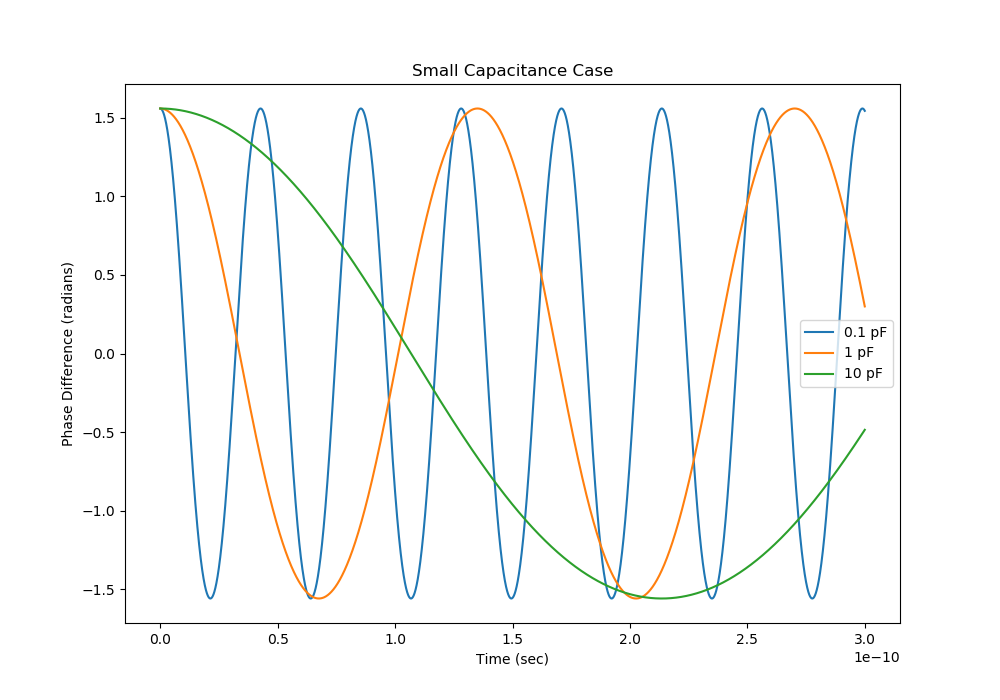
\includegraphics[scale=0.60]{uud-jjsmallc.png}
\end{center}
\end{figure}

\begin{figure}
\caption{Phase Difference of Nondriven-undamped Josephson Junction}
\begin{center}
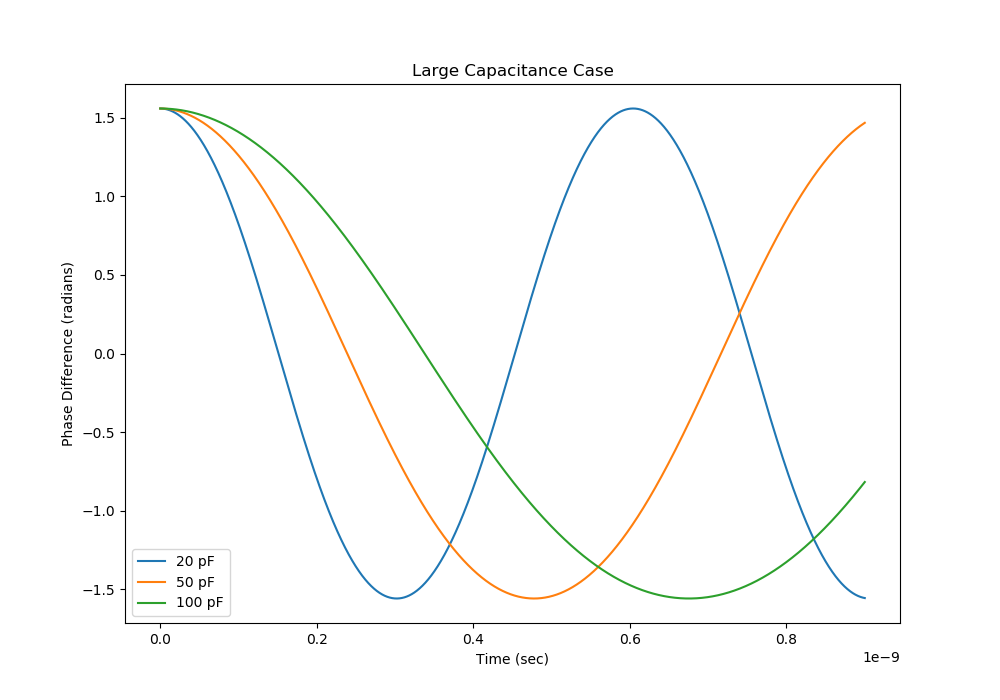
\includegraphics[scale=0.60]{uud-jjlargec.png}
\end{center}
\end{figure}


We note that the behavior of the circuit is approximately sinusoidal for smaller initial phase differences, but for cases where the initial phase difference is larger, the more rounded curve which one associates with the elliptic integral is visible.  It should also be noted that the frequency of the oscillations decreases when a larger initial phase is chosen.  Thus, a large phase difference actually excludes us from detecting smaller frequencies.  So, experimentally it is not advantageous to utilize a super large starting phase difference in the superconductors.

\begin{figure}
\caption{Phase Difference of Nondriven-undamped Josephson Junction}
\begin{center}
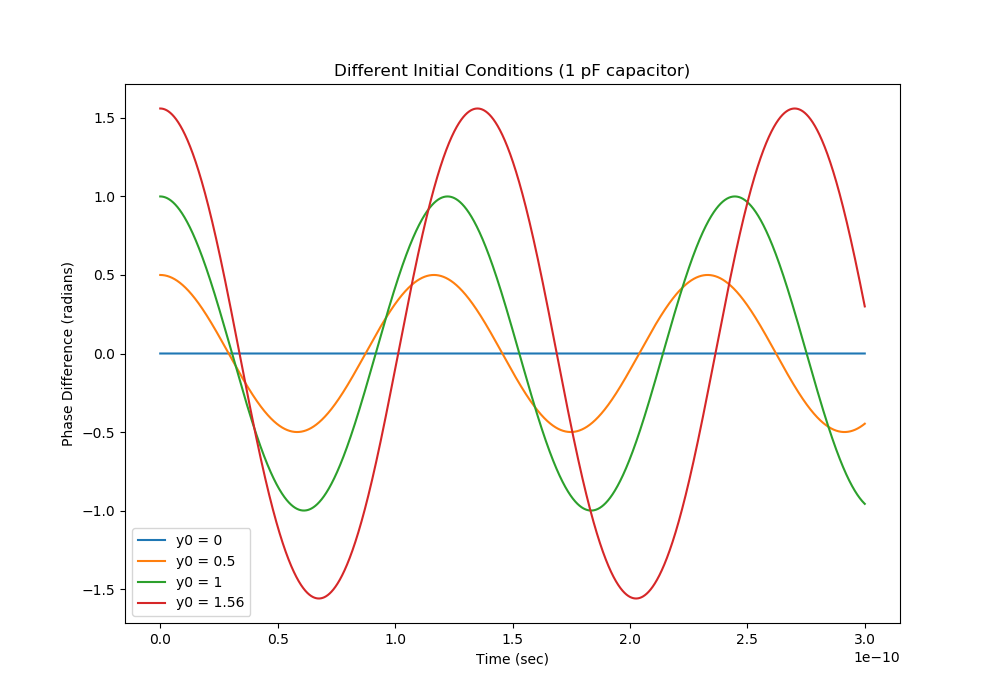
\includegraphics[scale=0.60]{uud-jjinit.png}
\end{center}
\end{figure}

\begin{figure}
\caption{Voltage Difference of Nondriven-undamped Josephson Junction}
\begin{center}
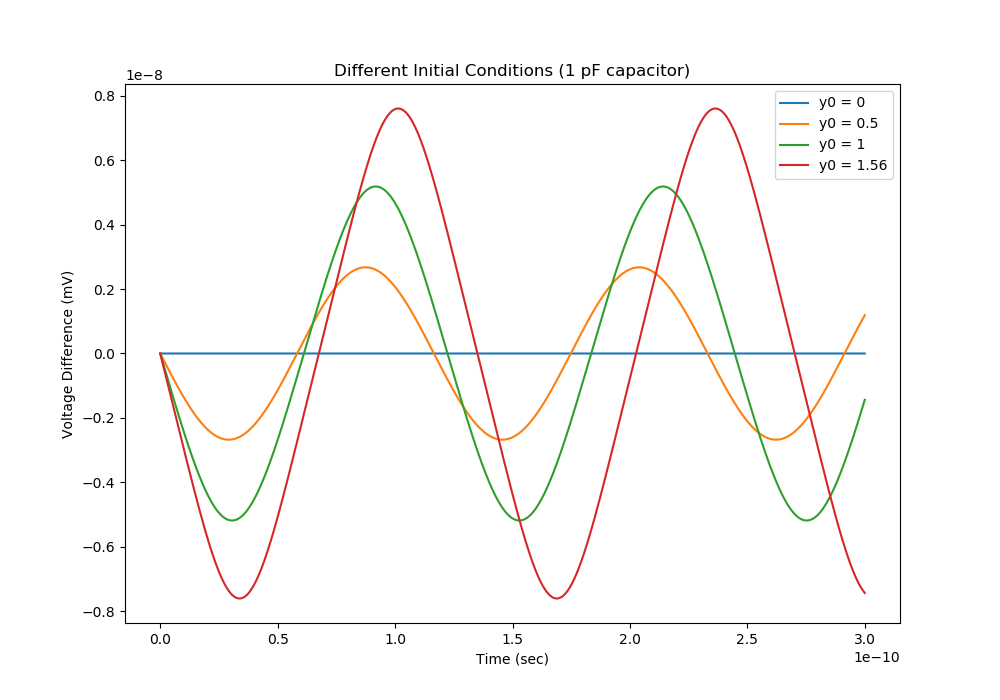
\includegraphics[scale=0.60]{uud-jjinitv.png}
\end{center}
\end{figure}


We now decide to inspect our system while it is under a constant driving current $I_b=1mA$, which is realistic and reminds one of the typical situation in which the Josephson Junction is implemented.  The curve we see is exactly what experiment shows, namely that there is some delay in the voltage over the capacitor, but shortly there is a small jump in voltage which turns into a linear function of time.  This shows the manner in which the undamped (no resistor version) of the Josephson Junction behaves.

\begin{equation}
\ddot{\phi}(t) + \dfrac{K}{C} I_c sin(\phi(t)) = \dfrac{K}{C} I_b
\end{equation}

\begin{figure}
\caption{Voltage Difference of Driven-undamped Josephson Junction}
\begin{center}
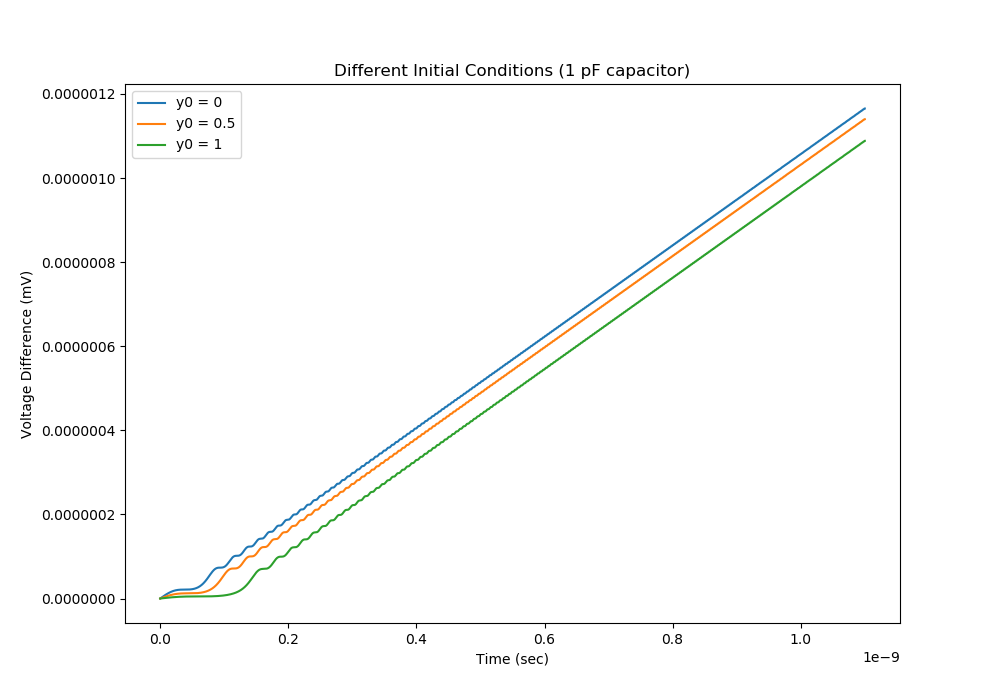
\includegraphics[scale=0.60]{ud-jjinitv.png}
\end{center}
\end{figure}

\subsubsection{The Damped Case}

In this case we do not consider the presence of the resistor negligible, thus we use the governing equation

\begin{equation}
\ddot{\phi}(t) + \dfrac{1}{RC} \dot{\phi}(t) + \dfrac{K}{C} I_c sin(\phi(t)) = \dfrac{K}{C} I(t)
\end{equation}

We notice that because of the scale of the problem that the value of the resistor only seems to have some apparent effect as we begin to drop below the $1 n\Omega$ mark.  Otherwise, the damping is not totally perceivable.

\begin{figure}
\caption{Phase Difference of Nondriven-damped Josephson Junction}
\begin{center}
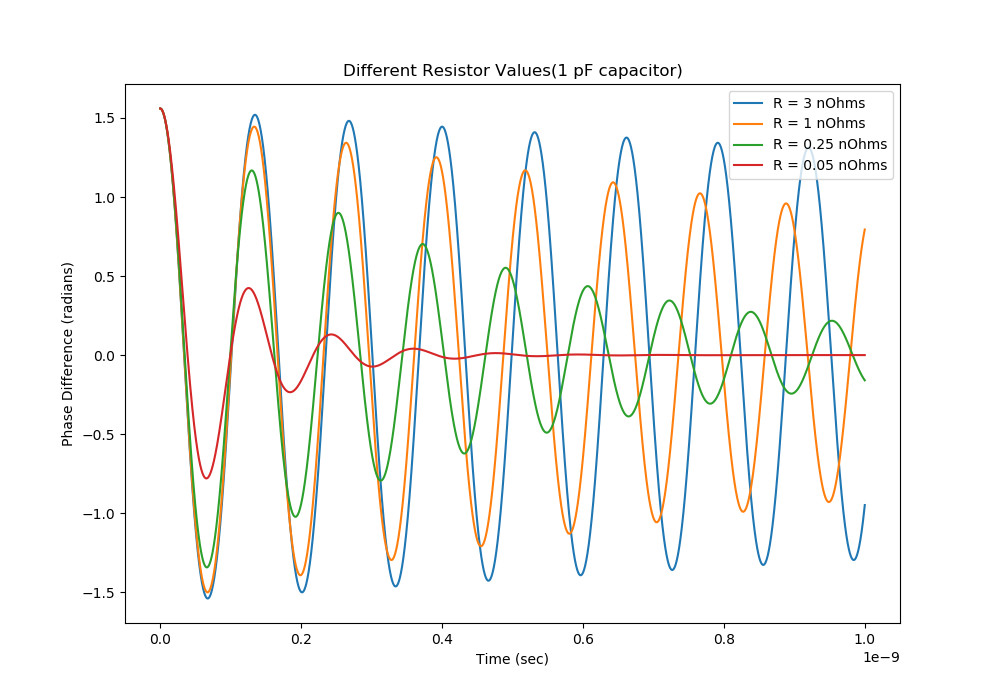
\includegraphics[scale=0.60]{dud-jjres.png}
\end{center}
\end{figure}

\begin{figure}
\caption{Voltage Difference of Nondriven-damped Josephson Junction}
\begin{center}
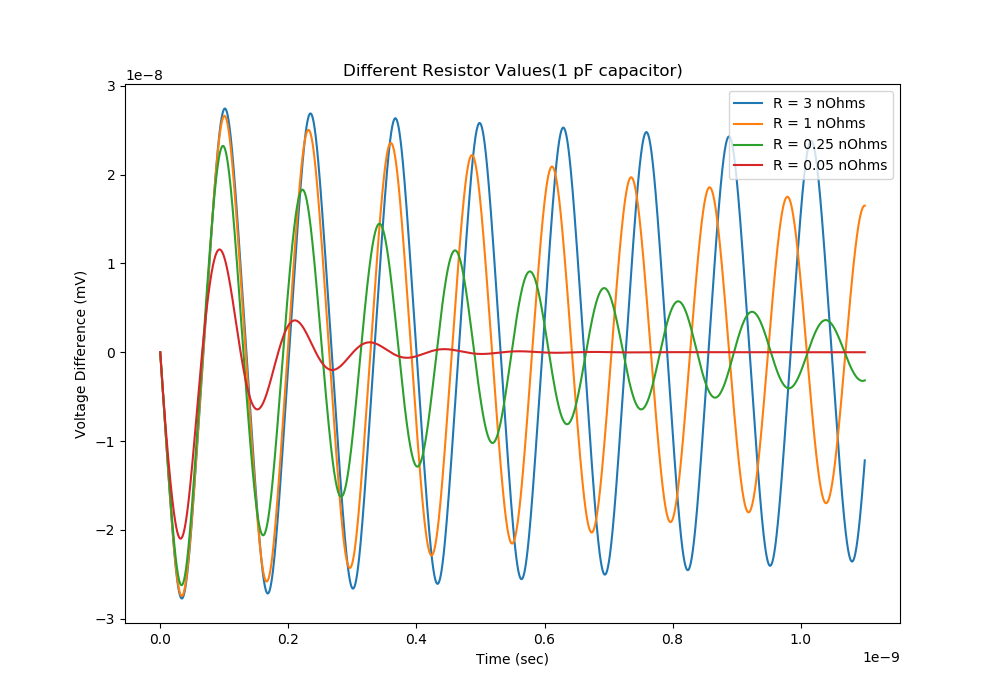
\includegraphics[scale=0.60]{dud-jjresv.png}
\end{center}
\end{figure}

Next we introduce a $1 mA$ driving current into the system and inspect how the different resistors make the corresponding phase differences and voltage differences change over time.  I noticed something very interesting which depended on the initial phase difference, which is that if the two superconducting materials started at a phase difference of $\pi / 2$ that there was relatively no change in the phase difference as time went on, where if one started with a low phase difference that the resulting solution increased incredibly fast.  Not only this, but the larger the damping force (ie. the smaller the resistance of the resistor) the less likely the solution was from becoming non zero.

\begin{figure}
\caption{Voltage Difference of Nondriven-damped J.J. $\Delta \phi_0 = \pi / 2$}
\begin{center}
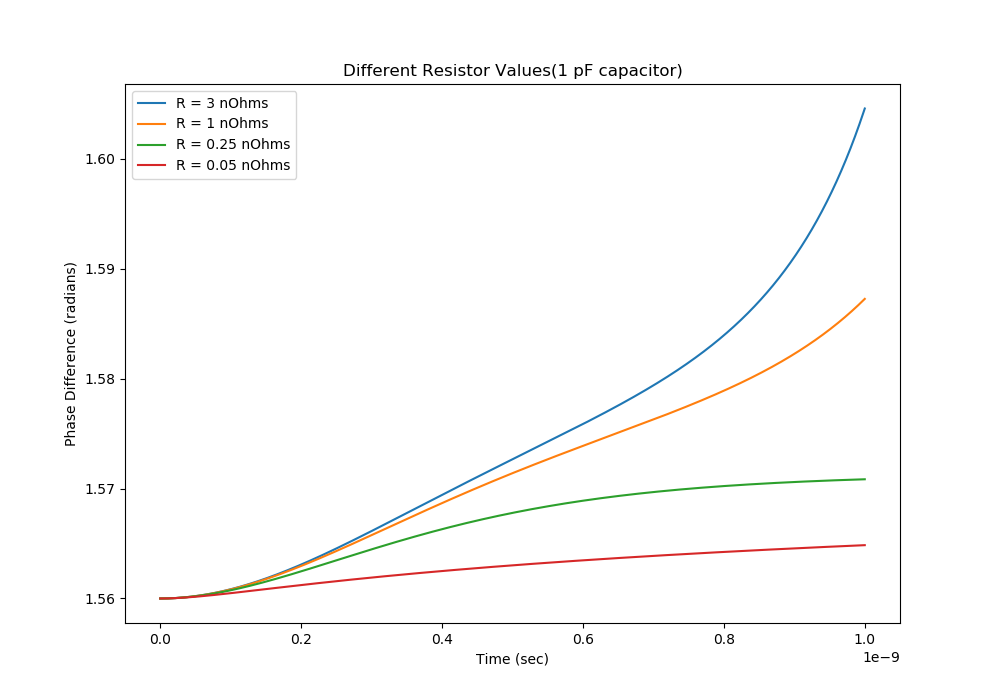
\includegraphics[scale=0.60]{dd-jjres.png}
\end{center}
\end{figure}

\begin{figure}
\caption{Voltage Difference of Nondriven-damped J.J. $\Delta \phi_0 = \pi / 2$}
\begin{center}
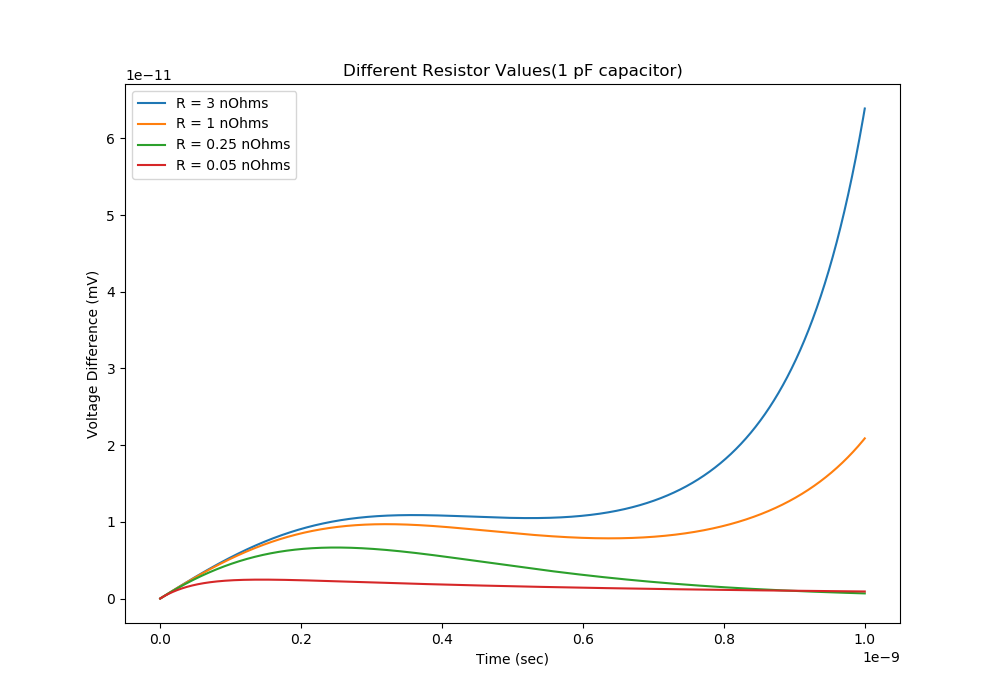
\includegraphics[scale=0.60]{dd-jjresv.png}
\end{center}
\end{figure}


\begin{figure}
\caption{Voltage Difference of Nondriven-damped J.J. $\Delta \phi_0 = 0$}
\begin{center}
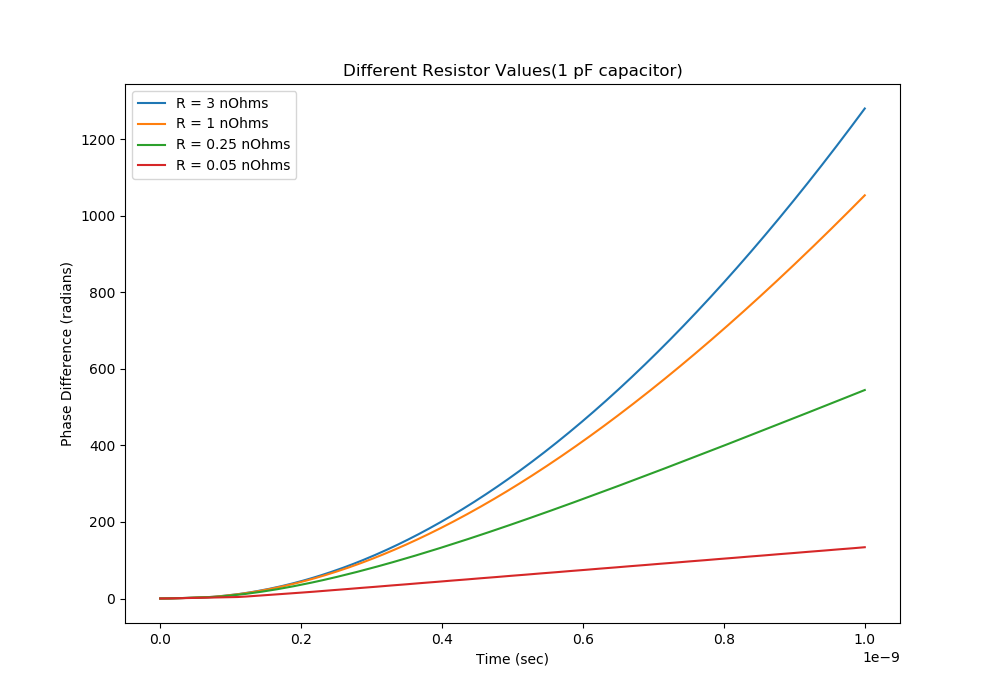
\includegraphics[scale=0.60]{dd-jjresphase0.png}
\end{center}
\end{figure}

\begin{figure}
\caption{Voltage Difference of Nondriven-damped J.J. $\Delta \phi_0 = 0$}
\begin{center}
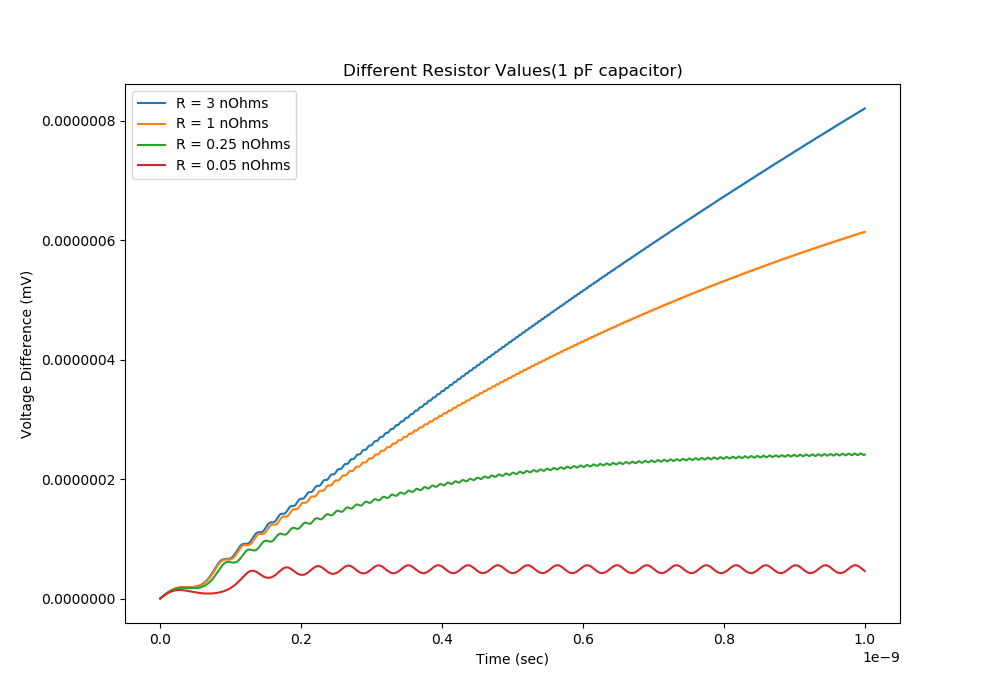
\includegraphics[scale=0.60]{dd-jjresphase0v.png}
\end{center}
\end{figure}

\end{document}



	